\scanpage{42}
\mspage{41}
% Top definitions; a note points to the bracketed adjective.
Catégorie des $k$-algèbres [\uline{graduées}] bivariantes \inserted{anticommutatives} (munies d'un degré $d(A)$, nulles en degré $\notin[1,d(A)]$; on ne donne pas de $\unsure{k_A|\kappa_A}:A\mathbin{-}k$).
\margin{\unsure{les hom sont homogènes.}}

Objet particulier de cette catégorie: $k$ de degré $0$.

Algèbre graduée bivariante \uline{jaugée}: muni d'un hom dans $k$.
Dans certains cas d'hom de telles, $f_*$ est déterminé par $f^*$. $(*)$

Produit tensoriel d'Algèbres bivariantes (resp. jaugées). Dans certains cas, c'est un produit dans la catégorie des Algèbres bivariantes jaugées.

% Middle: simplicial special case.
Algèbre graduée bivariante \inserted{(resp. gr. biv. jaugée)} \uline{simpliciale}. \deleted{\unsure{resp.}} Cas \uline{spécial}: on a
\[
A(I'\amalg I'')\xleftarrow[\sim]{(\alpha^*,\beta^*)}A(I')\otimes A(I''),
\]
d'autre part si $\alpha:I\mathbin{-}J$, $\beta:I'\longrightarrow J'$, sur $\alpha\amalg\beta=\gamma:I\amalg I'\mathbin{-}J\amalg J'$, on veut que $(\alpha\amalg\beta)_*:A(\unsure{J\amalg J'})\mathbin{-}A(I\amalg I')$ s'identifie à $\alpha_*\otimes\beta_*$. On voit que si $A(\Delta^0)=A_0$ est ``de Poincaré'' (cas jaugé) $A(\unsure{\bullet})\mathbin{-}A(\unsure{\varnothing|\omega})$ est \unsure{une jauge}, alors $A(\unsure{\bullet})$ est \unsure{Alg.} de Poincaré, et des alg. de Poincaré.

Et $A(\unsure{\bullet})\unsure{\mathbin{-}|\longmapsto}(A_0,\delta)$ est un foncteur pl. fidèle de la catégorie des Alg. graduées bivariantes jaugées simpliciales, dans la catégorie des algèbres \inserted{gr.} bivariantes jaugées $A$, munies d'un $\Delta\in[A\otimes A]^{d(A)}_{\unsure{0}}$ [il convient de préciser les axiomes à mettre sur ce $\Delta$]
\margin{\uline{à vérifier}; il faut d'abord voir qu'il suffit de connaître $\delta_*:A\longrightarrow A\otimes A$; \unsure{en posant} $\Delta=\delta_*(1)$}

% Example, with revisions and left marginal coefficient-field qualification.
\uuline{Ex} 1) Si on a une théorie ch. \deleted{\unsure{sur les variétés}} [satisfaisant Künneth et Poincaré)] sur la catégorie \inserted{$\unsure{\mathcal V|V}$} des variétés complètes algébriques non \uline{singulières} de dim $d$, \deleted{\unsure{sur un corps}} \inserted{sur un corps donné}, d'où un foncteur \inserted{cov} de $\unsure{\mathcal V|V}$ dans la catégorie $C_{\mathrm{jaug}}$ des Alg. gr. bivar. \uline{jaugées} sur $k$, et en \unsure{transformant} par ce foncteur l'objet simplicial canonique $I\longmapsto X^I$ défini par $X\in\unsure{\mathcal V|V}$, on trouve une Algèbre bivariante simpliciale bivariante jaugée canonique, d'ailleurs définie axiomatiquement, comme dit plus haut, par \unsure{sa composante} $H^*(X)$\ldots
\margin{$k$ un \uline{corps}}

\figure{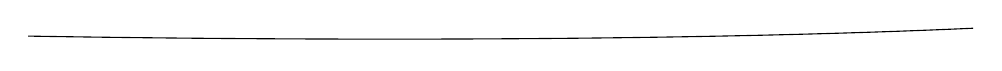
\begin{tikzpicture}\draw (0,0) .. controls (3,-.05) and (8,-.08) .. (12,.1);\end{tikzpicture}}
% Footnote corresponding to (*).
$(*)$ Attention, les \uline{isom} $(f^*,f_*)$ ne sont pas néc. tels que $f_*=f^{*-1}$ i.e. $f_*(1)=1$ ($\Rightarrow$ \deleted{\unsure{pas}} que $k_Af^*=k_B$), ex: $f^*=\mathrm{id}$, $f_*(y)=y\sigma$ $(\sigma\in A^*)$, $k_B(y)=k_A(y\sigma^{-1})$\ldots
